% Options for packages loaded elsewhere
\PassOptionsToPackage{unicode}{hyperref}
\PassOptionsToPackage{hyphens}{url}
\PassOptionsToPackage{dvipsnames,svgnames*,x11names*}{xcolor}
%
\documentclass[
  11pt,
  american,
  11pt,
  oneside]{scrreprt}
\usepackage{lmodern}
\usepackage{amssymb,amsmath}
\usepackage{ifxetex,ifluatex}
\ifnum 0\ifxetex 1\fi\ifluatex 1\fi=0 % if pdftex
  \usepackage[T1]{fontenc}
  \usepackage[utf8]{inputenc}
  \usepackage{textcomp} % provide euro and other symbols
\else % if luatex or xetex
  \usepackage{unicode-math}
  \defaultfontfeatures{Scale=MatchLowercase}
  \defaultfontfeatures[\rmfamily]{Ligatures=TeX,Scale=1}
\fi
% Use upquote if available, for straight quotes in verbatim environments
\IfFileExists{upquote.sty}{\usepackage{upquote}}{}
\IfFileExists{microtype.sty}{% use microtype if available
  \usepackage[]{microtype}
  \UseMicrotypeSet[protrusion]{basicmath} % disable protrusion for tt fonts
}{}
\makeatletter
\@ifundefined{KOMAClassName}{% if non-KOMA class
  \IfFileExists{parskip.sty}{%
    \usepackage{parskip}
  }{% else
    \setlength{\parindent}{0pt}
    \setlength{\parskip}{6pt plus 2pt minus 1pt}}
}{% if KOMA class
  \KOMAoptions{parskip=half}}
\makeatother
\usepackage{xcolor}
\IfFileExists{xurl.sty}{\usepackage{xurl}}{} % add URL line breaks if available
\IfFileExists{bookmark.sty}{\usepackage{bookmark}}{\usepackage{hyperref}}
\hypersetup{
  pdftitle={From StableHLO to Tensix},
  pdfauthor={libtt technical report},
  pdflang={en-US},
  pdfkeywords={libtt, Tenstorrent, PJRT, TT-MLIR, TT-Metalium, Blackhole, Qwen3, LLM
inference, compiler optimization, kernel fusion},
  colorlinks=true,
  linkcolor=MidnightBlue,
  filecolor=Maroon,
  citecolor=Blue,
  urlcolor=MidnightBlue,
  pdfcreator={LaTeX via pandoc}}
\urlstyle{same} % disable monospaced font for URLs
\usepackage[margin=25mm]{geometry}
\usepackage{color}
\usepackage{fancyvrb}
\newcommand{\VerbBar}{|}
\newcommand{\VERB}{\Verb[commandchars=\\\{\}]}
\DefineVerbatimEnvironment{Highlighting}{Verbatim}{commandchars=\\\{\}}
% Add ',fontsize=\small' for more characters per line
\newenvironment{Shaded}{}{}
\newcommand{\AlertTok}[1]{\textcolor[rgb]{1.00,0.00,0.00}{\textbf{#1}}}
\newcommand{\AnnotationTok}[1]{\textcolor[rgb]{0.38,0.63,0.69}{\textbf{\textit{#1}}}}
\newcommand{\AttributeTok}[1]{\textcolor[rgb]{0.49,0.56,0.16}{#1}}
\newcommand{\BaseNTok}[1]{\textcolor[rgb]{0.25,0.63,0.44}{#1}}
\newcommand{\BuiltInTok}[1]{#1}
\newcommand{\CharTok}[1]{\textcolor[rgb]{0.25,0.44,0.63}{#1}}
\newcommand{\CommentTok}[1]{\textcolor[rgb]{0.38,0.63,0.69}{\textit{#1}}}
\newcommand{\CommentVarTok}[1]{\textcolor[rgb]{0.38,0.63,0.69}{\textbf{\textit{#1}}}}
\newcommand{\ConstantTok}[1]{\textcolor[rgb]{0.53,0.00,0.00}{#1}}
\newcommand{\ControlFlowTok}[1]{\textcolor[rgb]{0.00,0.44,0.13}{\textbf{#1}}}
\newcommand{\DataTypeTok}[1]{\textcolor[rgb]{0.56,0.13,0.00}{#1}}
\newcommand{\DecValTok}[1]{\textcolor[rgb]{0.25,0.63,0.44}{#1}}
\newcommand{\DocumentationTok}[1]{\textcolor[rgb]{0.73,0.13,0.13}{\textit{#1}}}
\newcommand{\ErrorTok}[1]{\textcolor[rgb]{1.00,0.00,0.00}{\textbf{#1}}}
\newcommand{\ExtensionTok}[1]{#1}
\newcommand{\FloatTok}[1]{\textcolor[rgb]{0.25,0.63,0.44}{#1}}
\newcommand{\FunctionTok}[1]{\textcolor[rgb]{0.02,0.16,0.49}{#1}}
\newcommand{\ImportTok}[1]{#1}
\newcommand{\InformationTok}[1]{\textcolor[rgb]{0.38,0.63,0.69}{\textbf{\textit{#1}}}}
\newcommand{\KeywordTok}[1]{\textcolor[rgb]{0.00,0.44,0.13}{\textbf{#1}}}
\newcommand{\NormalTok}[1]{#1}
\newcommand{\OperatorTok}[1]{\textcolor[rgb]{0.40,0.40,0.40}{#1}}
\newcommand{\OtherTok}[1]{\textcolor[rgb]{0.00,0.44,0.13}{#1}}
\newcommand{\PreprocessorTok}[1]{\textcolor[rgb]{0.74,0.48,0.00}{#1}}
\newcommand{\RegionMarkerTok}[1]{#1}
\newcommand{\SpecialCharTok}[1]{\textcolor[rgb]{0.25,0.44,0.63}{#1}}
\newcommand{\SpecialStringTok}[1]{\textcolor[rgb]{0.73,0.40,0.53}{#1}}
\newcommand{\StringTok}[1]{\textcolor[rgb]{0.25,0.44,0.63}{#1}}
\newcommand{\VariableTok}[1]{\textcolor[rgb]{0.10,0.09,0.49}{#1}}
\newcommand{\VerbatimStringTok}[1]{\textcolor[rgb]{0.25,0.44,0.63}{#1}}
\newcommand{\WarningTok}[1]{\textcolor[rgb]{0.38,0.63,0.69}{\textbf{\textit{#1}}}}
\usepackage{longtable,booktabs}
% Correct order of tables after \paragraph or \subparagraph
\usepackage{etoolbox}
\makeatletter
\patchcmd\longtable{\par}{\if@noskipsec\mbox{}\fi\par}{}{}
\makeatother
% Allow footnotes in longtable head/foot
\IfFileExists{footnotehyper.sty}{\usepackage{footnotehyper}}{\usepackage{footnote}}
\makesavenoteenv{longtable}
\usepackage{graphicx}
\makeatletter
\def\maxwidth{\ifdim\Gin@nat@width>\linewidth\linewidth\else\Gin@nat@width\fi}
\def\maxheight{\ifdim\Gin@nat@height>\textheight\textheight\else\Gin@nat@height\fi}
\makeatother
% Scale images if necessary, so that they will not overflow the page
% margins by default, and it is still possible to overwrite the defaults
% using explicit options in \includegraphics[width, height, ...]{}
\setkeys{Gin}{width=\maxwidth,height=\maxheight,keepaspectratio}
% Set default figure placement to htbp
\makeatletter
\def\fps@figure{htbp}
\makeatother
\setlength{\emergencystretch}{3em} % prevent overfull lines
\providecommand{\tightlist}{%
  \setlength{\itemsep}{0pt}\setlength{\parskip}{0pt}}
\setcounter{secnumdepth}{3}
\usepackage{microtype}
\usepackage{booktabs}
\usepackage{longtable}
\usepackage{graphicx}
\usepackage{xcolor}
\usepackage{caption}
\definecolor{MidnightBlue}{HTML}{005F73}
\definecolor{AccentOrange}{HTML}{E29578}
\setlength{\emergencystretch}{3em}
\setkomafont{disposition}{\color{MidnightBlue}}
\ifxetex
  % Load polyglossia as late as possible: uses bidi with RTL langages (e.g. Hebrew, Arabic)
  \usepackage{polyglossia}
  \setmainlanguage[variant=american]{english}
\else
  \usepackage[shorthands=off,main=american]{babel}
\fi

\title{From StableHLO to Tensix}
\usepackage{etoolbox}
\makeatletter
\providecommand{\subtitle}[1]{% add subtitle to \maketitle
  \apptocmd{\@title}{\par {\large #1 \par}}{}{}
}
\makeatother
\subtitle{libtt as a hermetic, full-stack runtime for Tenstorrent
accelerators}
\author{libtt technical report}
\date{15 July 2026}

\begin{document}
\maketitle

{
\hypersetup{linkcolor=}
\setcounter{tocdepth}{3}
\tableofcontents
}
\hypertarget{abstract}{%
\chapter*{Abstract}\label{abstract}}
\addcontentsline{toc}{chapter}{Abstract}

libtt packages the Tenstorrent JAX stack as one PJRT shared library. It
builds and pins TT-XLA {[}1{]}, TT-MLIR {[}2{]}, TTNN {[}3{]},
TT-Metalium {[}4{]}, device kernels, and runtime assets in
\texttt{libtt.so}. The target needs compatible drivers and firmware, but
no separate compiler or TT-Metal installation.

This report maps libtt's optimizations to StableHLO, TTIR, TTNN, D2M,
TTKernel, TTMetal, the runtime, and device kernels. It is organized by
patch concept because one optimization often crosses several levels. For
example, the SwiGLU epilogue starts as graph recognition and ends as a
Dst-resident Tensix kernel.

On Qwen3-8B decode on a Blackhole P150, the established optimization
line raises end-to-end throughput from 16.265 to 26.123 tokens/s
(+60.61\%). A 110-core down projection adds 5.96\% pure decode
throughput, reaches 27.753 tokens/s, and cuts kernel time from 217.188
to 154.932 microseconds per layer. Against a matched 32-sample
tt-inference-server v0.10.0 run {[}25{]}, current libtt is 11.51\%
faster in pure decode and 11.48\% faster end to end. Increasing the
SwiGLU K block from two to four tiles changes throughput by only
+0.27\%.

\hypertarget{executive-summary}{%
\chapter*{Executive summary}\label{executive-summary}}
\addcontentsline{toc}{chapter}{Executive summary}

\texttt{libtt.so} contains the TT-XLA PJRT implementation, TT-MLIR
compiler, TTNN and TT-Metal runtime code, and a compressed archive of
TT-Metal runtime assets. It extracts the archive on first load. This
deployment model resembles Google's \texttt{libtpu.so}, which contains
the TPU compiler, driver, and hardware communication code {[}7{]}.

One Bazel build pins the source revisions, applies the patch series, and
builds the shared library. Its tools and dependencies are explicit
inputs, following Bazel's definition of a hermetic build {[}8{]}. A
compiler rewrite, runtime change, and device kernel can therefore be
built and benchmarked together.

The measured work supports six conclusions:

\begin{enumerate}
\def\labelenumi{\arabic{enumi}.}
\tightlist
\item
  \textbf{Recover model semantics before lowering.} TTIR and TTNN
  patterns recover RMSNorm, SiLU, and QKV structure from primitive JAX
  operations. The foundation group adds 22.58\%; SiLU recognition adds
  3.30\%; QKV fusion adds 1.15\%.
\item
  \textbf{Use the runtime for shape-dependent layouts.} Width-sharding
  one-token RMSNorm across 16 cores adds 13.61\%.
\item
  \textbf{Fuse at the producer boundary.} Combining gate/up matmuls
  alone changes throughput by -1.69\%. Consumer-side SiLU fusion changes
  it by -0.65\%. A matmul-SwiGLU epilogue that keeps both results in Dst
  adds 2.73\%.
\item
  \textbf{Measure blocking choices.} Increasing the SwiGLU K block from
  two to four tiles changes throughput by +0.27\%, so two remains the
  default.
\item
  \textbf{Use more cores without rereading weights.} The 110-core down
  projection raises effective BFP8 bandwidth from 246.2 to 345.2 GB/s,
  cuts kernel time by 28.7\%, and adds 5.96\% pure decode throughput.
\item
  \textbf{Trace short prefill.} Capturing the one-tile prefill graph
  reduces mean time to first token from 618.84 to 59.15 ms and improves
  the primary 128-token benchmark by 10.23\%. Pure decode changes by
  +0.36\%.
\end{enumerate}

The current build reaches 27.753 decode tokens/s and 27.619 streaming
end-to-end tokens/s. The matched TTIS reference reaches 24.887 and
24.776 tokens/s, respectively.

\begin{figure}
\hypertarget{fig:stack}{%
\centering
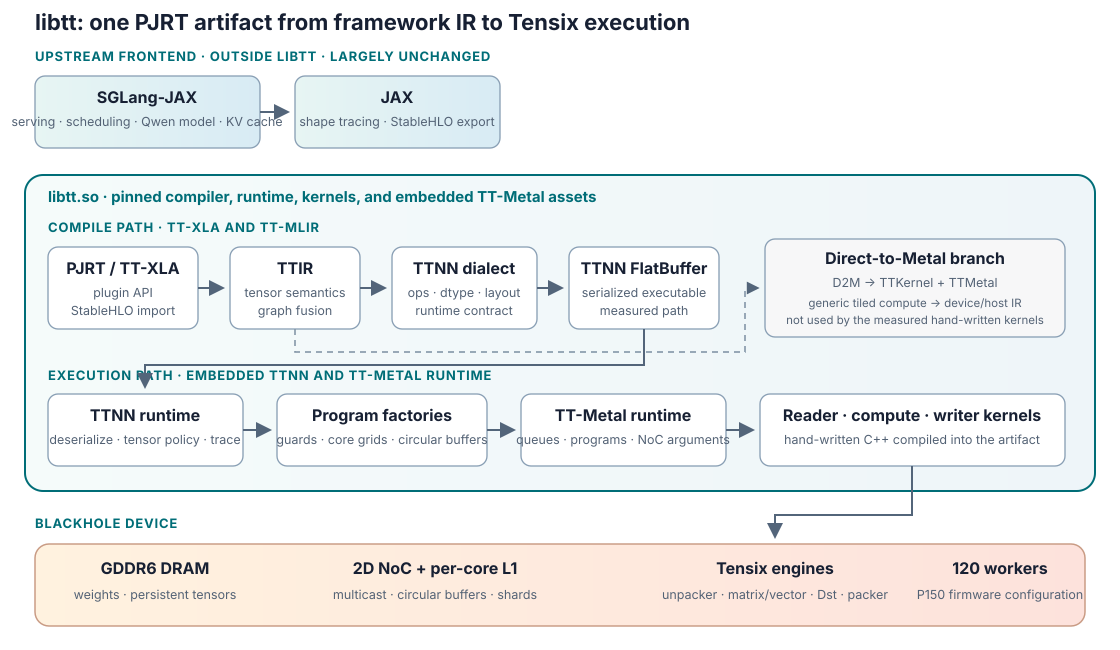
\includegraphics[width=1\textwidth,height=\textheight]{figures/stack.svg}
\caption{libtt's serving, compilation, runtime, and device
layers.}\label{fig:stack}
}
\end{figure}

\hypertarget{design}{%
\chapter{Design}\label{design}}

\hypertarget{deployment-model}{%
\section{Deployment model}\label{deployment-model}}

PJRT lets frameworks call device-specific plugins through one interface
{[}9{]}. libtt implements that interface for Tenstorrent:

\begin{verbatim}
JAX process
  `-- dynamically loads libtt.so through PJRT
       |-- compiles StableHLO for Tenstorrent
       |-- allocates and transfers device buffers
       |-- loads and executes serialized TTNN programs
       `-- initializes the embedded TT-Metal runtime assets
\end{verbatim}

libtt's C++ glue extracts the embedded archive to a fingerprinted
temporary directory, sets \texttt{TT\_METAL\_RUNTIME\_ROOT} before PJRT
starts, links the upstream plugin, and exports only the PJRT entry
points. Most code comes from pinned open-source dependencies and the
applied patch series.

The compiler and TT-Metal runtime do not need to be installed on the
target. With compatible drivers and firmware, \texttt{libtt.so} contains
the software needed to compile and run JAX programs. This is the
intended similarity to \texttt{libtpu.so} {[}7{]}.

\hypertarget{one-build-graph}{%
\section{One build graph}\label{one-build-graph}}

libtt uses Bazel modules and repository rules to pin TT-UMD {[}5{]},
SFPI {[}6{]}, TT-Metal, LLVM, StableHLO, TT-XLA, TT-MLIR, Shardy, and
supporting C++ libraries. Bazel overlays add targets for projects that
use another build system. The \texttt{//:tt} target produces
\texttt{bazel-bin/libtt.so}.

This organization has three practical effects:

\begin{itemize}
\tightlist
\item
  Source revisions, overlays, patches, toolchains, and link rules are
  inputs to one build.
\item
  Compiler, schema, runtime, program-factory, and kernel changes can be
  tested together.
\item
  An agent can inspect and edit every layer in one workspace, rebuild
  one target, and run one benchmark.
\end{itemize}

Tenstorrent's compiler overview describes the same open path from
framework frontends through TT-MLIR dialects to TT-Metalium {[}12,
13{]}. libtt builds a pinned part of that path as one artifact.

\hypertarget{cross-layer-changes}{%
\section{Cross-layer changes}\label{cross-layer-changes}}

The matmul-SwiGLU epilogue crosses six layers:

\begin{enumerate}
\def\labelenumi{\arabic{enumi}.}
\tightlist
\item
  A graph pass must prove that a paired gate/up matmul feeds the exact
  \texttt{silu(gate)\ *\ up} expression.
\item
  TTNN IR needs an operation-level representation that preserves the
  fused semantic through lowering.
\item
  The serialized executable needs to carry the new matmul attribute.
\item
  The runtime must dispatch that operation into TTNN.
\item
  TTNN must select a program factory only for supported shapes, dtypes,
  layouts, and hardware.
\item
  Reader, compute, and writer kernels must keep the paired tiles
  resident in Dst and emit only the half-width final result.
\end{enumerate}

These steps form one patch concept even though they touch several
abstraction levels and two upstream repositories.

\hypertarget{compilation-and-execution-architecture}{%
\chapter{Compilation and execution
architecture}\label{compilation-and-execution-architecture}}

\hypertarget{the-framework-boundary-jax-stablehlo-and-pjrt}{%
\section{The framework boundary: JAX, StableHLO, and
PJRT}\label{the-framework-boundary-jax-stablehlo-and-pjrt}}

SGLang-JAX owns serving, tokenization, scheduling, the JAX Qwen model,
and the paged KV cache {[}21{]}. JAX traces each shape-specific
computation to StableHLO, a portable operation set between frameworks
and compilers {[}10{]}. PJRT hides the device-specific compiler and
runtime from JAX {[}9{]}.

The steady-state request path is:

\begin{verbatim}
SGLang-JAX → JAX trace → StableHLO → libtt/PJRT
            → TT-XLA → TT-MLIR → TTNN executable
            → TTNN runtime → TT-Metal programs → Blackhole
\end{verbatim}

\texttt{libtt.so} accepts StableHLO and executes a serialized TTNN
program.

\hypertarget{tt-mlir-ir-levels}{%
\section{TT-MLIR IR levels}\label{tt-mlir-ir-levels}}

MLIR supports dialects at different abstraction levels {[}11{]}. TT-MLIR
uses them for model semantics, layouts, tiled computation, device
kernels, and host/device control {[}13{]}. Each optimization should use
the highest level that still has the information it needs.

\begin{longtable}[]{@{}lll@{}}
\caption{The TT-MLIR IR ladder and where libtt's measured path uses
it.}\tabularnewline
\toprule
\begin{minipage}[b]{0.30\columnwidth}\raggedright
Representation\strut
\end{minipage} & \begin{minipage}[b]{0.30\columnwidth}\raggedright
Abstraction and purpose\strut
\end{minipage} & \begin{minipage}[b]{0.30\columnwidth}\raggedright
Relationship to current libtt optimizations\strut
\end{minipage}\tabularnewline
\midrule
\endfirsthead
\toprule
\begin{minipage}[b]{0.30\columnwidth}\raggedright
Representation\strut
\end{minipage} & \begin{minipage}[b]{0.30\columnwidth}\raggedright
Abstraction and purpose\strut
\end{minipage} & \begin{minipage}[b]{0.30\columnwidth}\raggedright
Relationship to current libtt optimizations\strut
\end{minipage}\tabularnewline
\midrule
\endhead
\begin{minipage}[t]{0.30\columnwidth}\raggedright
\textbf{StableHLO}\strut
\end{minipage} & \begin{minipage}[t]{0.30\columnwidth}\raggedright
Framework-portable tensor graph with specified operation semantics
{[}10{]}.\strut
\end{minipage} & \begin{minipage}[t]{0.30\columnwidth}\raggedright
Input to TT-XLA/TT-MLIR. Framework algebra such as expanded SiLU is
visible here and after import, but libtt's patches generally match it in
TTIR/TTNN passes.\strut
\end{minipage}\tabularnewline
\begin{minipage}[t]{0.30\columnwidth}\raggedright
\textbf{TTIR}\strut
\end{minipage} & \begin{minipage}[t]{0.30\columnwidth}\raggedright
Hardware-aware, high-level tensor IR. It preserves named tensor
operations while permitting fusion and canonicalization before a
concrete runtime API is chosen {[}13{]}.\strut
\end{minipage} & \begin{minipage}[t]{0.30\columnwidth}\raggedright
JAX RMSNorm recognition, expanded-SiLU recovery, shared-LHS matmul
grouping, role propagation, and part of QKV/RoPE fusion.\strut
\end{minipage}\tabularnewline
\begin{minipage}[t]{0.30\columnwidth}\raggedright
\textbf{TTNN dialect}\strut
\end{minipage} & \begin{minipage}[t]{0.30\columnwidth}\raggedright
High-level tensor IR designed to model the TTNN library closely. Its
types and attributes carry tiled layouts, memory spaces, sharding, and
device data types {[}13, 14{]}.\strut
\end{minipage} & \begin{minipage}[t]{0.30\columnwidth}\raggedright
QKV composite fusion, \texttt{matmul\_swiglu}, layout selection, cache
return types, and lowering to the serialized TTNN operation graph.\strut
\end{minipage}\tabularnewline
\begin{minipage}[t]{0.30\columnwidth}\raggedright
\textbf{TTNN FlatBuffer}\strut
\end{minipage} & \begin{minipage}[t]{0.30\columnwidth}\raggedright
Serialized executable operation graph consumed by the TTNN runtime. It
is an artifact rather than an MLIR dialect.\strut
\end{minipage} & \begin{minipage}[t]{0.30\columnwidth}\raggedright
Carries operation parameters such as the fused-SwiGLU matmul flag across
the compiler/runtime boundary.\strut
\end{minipage}\tabularnewline
\begin{minipage}[t]{0.30\columnwidth}\raggedright
\textbf{D2M dialect}\strut
\end{minipage} & \begin{minipage}[t]{0.30\columnwidth}\raggedright
Generic tensor/memref computation analogous to \texttt{linalg.generic},
augmented with grids, sharded tensors, circular buffers, and explicit
data movement {[}13{]}.\strut
\end{minipage} & \begin{minipage}[t]{0.30\columnwidth}\raggedright
An alternative direct-to-metal route. The measured custom SwiGLU and
down-projection kernels are hand-written TT-Metal/TTNN patches, so they
do \textbf{not} pass through D2M.\strut
\end{minipage}\tabularnewline
\begin{minipage}[t]{0.30\columnwidth}\raggedright
\textbf{TTKernel dialect}\strut
\end{minipage} & \begin{minipage}[t]{0.30\columnwidth}\raggedright
Low-level device-kernel IR exposing circular buffers, tile registers,
NoC transactions, and synchronization with an intended near one-to-one
mapping to TT-Metal kernels {[}13{]}.\strut
\end{minipage} & \begin{minipage}[t]{0.30\columnwidth}\raggedright
Relevant to generated direct-to-metal kernels; not the representation of
the hand-written C++ kernels measured here.\strut
\end{minipage}\tabularnewline
\begin{minipage}[t]{0.30\columnwidth}\raggedright
\textbf{TTMetal dialect}\strut
\end{minipage} & \begin{minipage}[t]{0.30\columnwidth}\raggedright
Host/device interop IR for allocation, transfers, program creation, and
enqueue operations {[}13{]}.\strut
\end{minipage} & \begin{minipage}[t]{0.30\columnwidth}\raggedright
Part of the direct-to-metal compiler route. The measured TTNN route
instead invokes TT-Metal host APIs from the TTNN runtime.\strut
\end{minipage}\tabularnewline
\bottomrule
\end{longtable}

The main lowering branch in this report is therefore:

\begin{verbatim}
StableHLO → TTIR → TTNN dialect → TTNN FlatBuffer
                                      ↓
                              TTNN C++ runtime
                                      ↓
                       TT-Metal host + C++ kernels
\end{verbatim}

TT-MLIR also supports the lower-level branch:

\begin{verbatim}
TTIR → D2M → TTKernel + TTMetal → generated device/host program
\end{verbatim}

Only the first branch runs the benchmarked patches. Their hand-written
C++ program factories and kernels are not TTKernel IR optimizations.

\hypertarget{ttnn-runtime-and-the-serialized-executable}{%
\section{TTNN runtime and the serialized
executable}\label{ttnn-runtime-and-the-serialized-executable}}

TTNN IR models operations such as matmul, RMSNorm, SDPA, and reshape.
Lowering serializes them into a FlatBuffer. The runtime deserializes the
graph, creates tensors, sets memory configurations, validates each
operation, and selects a program factory. The RMSNorm patch uses the
concrete input shape here to choose a 16-core width-sharded layout; the
compiler still emits a normal RMSNorm.

\hypertarget{tt-metal-programs-and-tensix-kernels}{%
\section{TT-Metal programs and Tensix
kernels}\label{tt-metal-programs-and-tensix-kernels}}

TT-Metalium uses cooperative dataflow rather than a GPU thread hierarchy
{[}15{]}. A program usually has:

\begin{itemize}
\tightlist
\item
  a reader data-movement kernel to fetch tiles from DRAM or another core
  into L1 circular buffers;
\item
  a compute kernel to unpack tiles, drive matrix/vector engines, and
  create result tiles; and
\item
  a writer data-movement kernel to drain result buffers to their
  destination.
\end{itemize}

Circular buffers are bounded queues shared by the threads of a Tensix
core {[}17{]}. Reader, compute, and writer kernels can overlap on
different tiles when their buffer and semaphore protocols are correct.

The compute engine exposes SrcA, SrcB, and Dst register sets. Matrix
results land in Dst; vector operations can transform them; the packer
writes them to an L1 circular buffer {[}16{]}. With 16-bit Dst storage
and double buffering enabled, the active half contains eight 32-by-32
tiles. That capacity determines the successful SwiGLU geometry: four
gate and four up tiles fill Dst exactly.

\hypertarget{tiles-memory-and-low-precision-weights}{%
\section{Tiles, memory, and low-precision
weights}\label{tiles-memory-and-low-precision-weights}}

TTNN's standard tile is 32 by 32 elements with four 16-by-16 faces
{[}18{]}. Final dimensions are padded, so batch-one decode still
presents a full tile row. Kernels must account for both the logical and
padded shapes.

Large weights reside in device DRAM; L1 is smaller, faster, and private
to each worker. TTNN \texttt{MemoryConfig} values describe interleaved
or sharded storage and DRAM or L1 placement. TT-MLIR layout attributes
similarly encode how a logical tensor maps to devices, cores, physical
shards, memory space, and padding {[}14{]}.

The benchmark uses BF16 activations and outputs with BFLOAT8\_B weights.
BFLOAT8\_B is block floating point: 16 values share an exponent
{[}19{]}. It reduces the dominant weight traffic in batch-one decode,
with a precision and packing trade-off. The custom matmuls use BF16
packer-L1 accumulation: partial sums are packed into an L1 slot and
reloaded for later K blocks, leaving Dst available for the current
block's tile group.

\hypertarget{decode-bottlenecks}{%
\section{Decode bottlenecks}\label{decode-bottlenecks}}

Qwen3 is a decoder-only Transformer family {[}22{]}. A simplified layer
is:

\[
\begin{aligned}
u &= \operatorname{RMSNorm}(h),\\
h' &= h + \operatorname{Attention}(Q(u),K(u),V(u);K_{cache},V_{cache}),\\
v &= \operatorname{RMSNorm}(h'),\\
g &= vW_{gate}, \qquad r = vW_{up},\\
h_{next} &= h' + \bigl(\operatorname{SiLU}(g)\odot r\bigr)W_{down}.
\end{aligned}
\]

RMSNorm and SwiGLU are standard model concepts {[}23, 24{]}. Prefill
shares each weight read across many rows. Serial decode applies a
logical \(1\times K\) by \(K\times N\) projection for every token, so
weight traffic and intermediate materialization dominate. The main
optimizations add width parallelism, reduce DRAM traffic, or avoid
packing an intermediate from Dst.

\hypertarget{optimization-map-by-patch-and-concept}{%
\chapter{Optimization map by patch and
concept}\label{optimization-map-by-patch-and-concept}}

Git revisions remain in the data files. The table groups changes by
patch concept and implementation level.

\begingroup\footnotesize

\begin{longtable}[]{@{}llr@{}}
\caption{Current model-path optimization concepts, implementation
levels, and measured effects.}\tabularnewline
\toprule
\begin{minipage}[b]{0.30\columnwidth}\raggedright
Concept\strut
\end{minipage} & \begin{minipage}[b]{0.30\columnwidth}\raggedright
Principal level / IR\strut
\end{minipage} & \begin{minipage}[b]{0.30\columnwidth}\raggedleft
Measured effect\strut
\end{minipage}\tabularnewline
\midrule
\endfirsthead
\toprule
\begin{minipage}[b]{0.30\columnwidth}\raggedright
Concept\strut
\end{minipage} & \begin{minipage}[b]{0.30\columnwidth}\raggedright
Principal level / IR\strut
\end{minipage} & \begin{minipage}[b]{0.30\columnwidth}\raggedleft
Measured effect\strut
\end{minipage}\tabularnewline
\midrule
\endhead
\begin{minipage}[t]{0.30\columnwidth}\raggedright
Recover JAX RMSNorm\strut
\end{minipage} & \begin{minipage}[t]{0.30\columnwidth}\raggedright
TTIR graph rewrite\strut
\end{minipage} & \begin{minipage}[t]{0.30\columnwidth}\raggedleft
Included in +22.58\% foundation bundle\strut
\end{minipage}\tabularnewline
\begin{minipage}[t]{0.30\columnwidth}\raggedright
Recognize expanded SiLU\strut
\end{minipage} & \begin{minipage}[t]{0.30\columnwidth}\raggedright
TTIR graph rewrite\strut
\end{minipage} & \begin{minipage}[t]{0.30\columnwidth}\raggedleft
+3.30\%\strut
\end{minipage}\tabularnewline
\begin{minipage}[t]{0.30\columnwidth}\raggedright
Fuse rank-3 decode RoPE\strut
\end{minipage} & \begin{minipage}[t]{0.30\columnwidth}\raggedright
TTIR/TTNN composite resolution\strut
\end{minipage} & \begin{minipage}[t]{0.30\columnwidth}\raggedleft
Included in foundation bundle\strut
\end{minipage}\tabularnewline
\begin{minipage}[t]{0.30\columnwidth}\raggedright
Fuse Qwen decode QKV structure\strut
\end{minipage} & \begin{minipage}[t]{0.30\columnwidth}\raggedright
TTIR ordering + TTNN fusion\strut
\end{minipage} & \begin{minipage}[t]{0.30\columnwidth}\raggedleft
+1.15\%\strut
\end{minipage}\tabularnewline
\begin{minipage}[t]{0.30\columnwidth}\raggedright
Preserve KV-cache result types\strut
\end{minipage} & \begin{minipage}[t]{0.30\columnwidth}\raggedright
TTNN type inference\strut
\end{minipage} & \begin{minipage}[t]{0.30\columnwidth}\raggedleft
Included in foundation bundle\strut
\end{minipage}\tabularnewline
\begin{minipage}[t]{0.30\columnwidth}\raggedright
Enable BF8 activation/weight path\strut
\end{minipage} & \begin{minipage}[t]{0.30\columnwidth}\raggedright
Compile options, TTNN lowering, host packing\strut
\end{minipage} & \begin{minipage}[t]{0.30\columnwidth}\raggedleft
Foundation/baseline; not isolated\strut
\end{minipage}\tabularnewline
\begin{minipage}[t]{0.30\columnwidth}\raggedright
Permit decode layouts\strut
\end{minipage} & \begin{minipage}[t]{0.30\columnwidth}\raggedright
TTNN/TT-Metal validation\strut
\end{minipage} & \begin{minipage}[t]{0.30\columnwidth}\raggedleft
Included in foundation bundle\strut
\end{minipage}\tabularnewline
\begin{minipage}[t]{0.30\columnwidth}\raggedright
Width-shard decode RMSNorm\strut
\end{minipage} & \begin{minipage}[t]{0.30\columnwidth}\raggedright
TTNN runtime policy\strut
\end{minipage} & \begin{minipage}[t]{0.30\columnwidth}\raggedleft
+13.61\%\strut
\end{minipage}\tabularnewline
\begin{minipage}[t]{0.30\columnwidth}\raggedright
Combine two shared-LHS matmuls\strut
\end{minipage} & \begin{minipage}[t]{0.30\columnwidth}\raggedright
TTIR fusion\strut
\end{minipage} & \begin{minipage}[t]{0.30\columnwidth}\raggedleft
-1.69\%; enables epilogue\strut
\end{minipage}\tabularnewline
\begin{minipage}[t]{0.30\columnwidth}\raggedright
True matmul-SwiGLU epilogue\strut
\end{minipage} & \begin{minipage}[t]{0.30\columnwidth}\raggedright
TTNN IR/FlatBuffer/runtime + TT-Metal\strut
\end{minipage} & \begin{minipage}[t]{0.30\columnwidth}\raggedleft
+2.73\%\strut
\end{minipage}\tabularnewline
\begin{minipage}[t]{0.30\columnwidth}\raggedright
Generalize and remove fallback\strut
\end{minipage} & \begin{minipage}[t]{0.30\columnwidth}\raggedright
TTNN matching/runtime simplification\strut
\end{minipage} & \begin{minipage}[t]{0.30\columnwidth}\raggedleft
-0.19\%\strut
\end{minipage}\tabularnewline
\begin{minipage}[t]{0.30\columnwidth}\raggedright
Sweep SwiGLU K blocking\strut
\end{minipage} & \begin{minipage}[t]{0.30\columnwidth}\raggedright
TT-Metal program and CB geometry\strut
\end{minipage} & \begin{minipage}[t]{0.30\columnwidth}\raggedleft
+0.27\%\strut
\end{minipage}\tabularnewline
\begin{minipage}[t]{0.30\columnwidth}\raggedright
Specialize down projection\strut
\end{minipage} & \begin{minipage}[t]{0.30\columnwidth}\raggedright
TTNN program selection + TT-Metal\strut
\end{minipage} & \begin{minipage}[t]{0.30\columnwidth}\raggedleft
+5.96\% pure decode\strut
\end{minipage}\tabularnewline
\begin{minipage}[t]{0.30\columnwidth}\raggedright
Trace one-tile prefill\strut
\end{minipage} & \begin{minipage}[t]{0.30\columnwidth}\raggedright
TTNN/TT-Metal runtime trace\strut
\end{minipage} & \begin{minipage}[t]{0.30\columnwidth}\raggedleft
-90.44\% TTFT; +10.23\% E2E\strut
\end{minipage}\tabularnewline
\bottomrule
\end{longtable}

\endgroup

Patch index:

\begingroup\scriptsize

\begin{verbatim}
RMSNorm graph       tt_mlir_fuse_jax_rms_norm.patch
expanded SiLU       tt_mlir_fuse_expanded_silu.patch
decode RoPE         tt_mlir_fuse_rank3_rope_decode.patch
QKV structure       tt_mlir_qwen_decode_qkv_projection_fusion.patch
KV-cache types      tt_mlir_kv_cache_dtype_return_types.patch
BF8 path            tt_mlir_single_chip_activation_dtype_lowering.patch
                    fast_bfloat16_bfp8_pack.patch
decode layouts      sdpa_decode_allow_l1_interleaved_q.patch
                    layernorm_allow_single_core_height_sharded.patch
RMSNorm sharding    tt_mlir_sharded_decode_rms_norm.patch
shared-LHS pair     tt_mlir_fuse_shared_lhs_matmul_pairs.patch
SwiGLU vertical     tt_mlir_fuse_matmul_swiglu.patch
                    matmul_swiglu_epilogue.patch
down projection     down_projection_110_core.patch
\end{verbatim}

\endgroup

The +22.58\% foundation figure combines patches that were not measured
separately. The blocking and down-projection tests use a streaming
decode clock, so they remain outside the cumulative sequence.

\hypertarget{recovering-model-semantics-in-ttir-and-ttnn}{%
\chapter{Recovering model semantics in TTIR and
TTNN}\label{recovering-model-semantics-in-ttir-and-ttnn}}

\hypertarget{rmsnorm-recognition}{%
\section{RMSNorm recognition}\label{rmsnorm-recognition}}

JAX can lower RMSNorm to square, reduce, epsilon addition, reciprocal
square root, scaling, and reshapes. A TTIR pattern proves this structure
and replaces it with one RMSNorm operation while the algebra and use-def
graph are still available. TTNN can then apply its normalization and
layout logic. Recognition is part of the foundation bundle and enables
the later runtime-sharding patch.

\hypertarget{expanded-silu-recognition}{%
\section{Expanded-SiLU recognition}\label{expanded-silu-recognition}}

The graph represents

\[
\operatorname{SiLU}(x)=x\,\sigma(x)=\frac{x}{1+\exp(-x)}
\]

with casts, broadcasts, reshapes, and a splatted scalar one.
\texttt{tt\_mlir\_fuse\_expanded\_silu.patch} looks through view-like
operations, verifies the constant and shared input, and replaces the
tree with SiLU. The isolated gain is \textbf{+3.30\%}.

\hypertarget{rank-3-rope-and-qkv-projection-structure}{%
\section{Rank-3 RoPE and QKV projection
structure}\label{rank-3-rope-and-qkv-projection-structure}}

Qwen projects Q, K, and V together, applies per-head RMSNorm to Q and K,
reshapes them by head count, and applies rotary position embedding. Two
patches recover this structure:

\begin{itemize}
\tightlist
\item
  \texttt{tt\_mlir\_fuse\_rank3\_rope\_decode.patch} accepts JAX's
  rank-3 decode form, temporarily maps it to the existing rank-4
  composite, and restores the expected result shape.
\item
  \texttt{tt\_mlir\_qwen\_decode\_qkv\_projection\_fusion.patch} orders
  projection roles, validates contiguous Q/K/V bounds, head counts, and
  head dimensions, and replaces materialized slices/reshapes with
  \texttt{nlp\_create\_qkv\_heads\_decode}. Q and K RMSNorm are
  recreated on the fused rank-4 results.
\end{itemize}

TTIR supplies candidate ordering and role information; TTNN owns the
composite operation and runtime contract. QKV fusion adds
\textbf{+1.15\%}. Rank-3 RoPE is part of the foundation bundle.

\hypertarget{kv-cache-dtype-and-role-propagation}{%
\section{KV-cache dtype and role
propagation}\label{kv-cache-dtype-and-role-propagation}}

KV-cache update operations are stateful boundaries. Their return types
must carry the selected device dtype, and graph-role metadata must
survive unary operations so later fusions can still identify query, key,
and value paths. The TT-MLIR and TT-XLA patches keep the low-precision
fused graph typed and recognizable. They are enabling changes rather
than isolated speedups.

\hypertarget{layout-precision-and-runtime-policy}{%
\chapter{Layout, precision, and runtime
policy}\label{layout-precision-and-runtime-policy}}

\hypertarget{bf8-lowering-and-fast-host-packing}{%
\section{BF8 lowering and fast host
packing}\label{bf8-lowering-and-fast-host-packing}}

The server requests \texttt{bfp\_bf8} for eligible weights. TT-XLA
enables single-chip lowering, TT-MLIR assigns the device dtype, and
TTNN/TT-Metal consume BFLOAT8\_B tiles.
\texttt{fast\_bfloat16\_bfp8\_pack.patch} speeds conversion of BF16 host
weights to 32-by-32 BFP8 tiles.

These changes attack two different phases:

\begin{itemize}
\tightlist
\item
  BF8 storage reduces steady-state device weight traffic during decode.
\item
  faster packing reduces model-load and preparation cost on the host.
\end{itemize}

The measurements do not isolate these effects from the foundation
bundle.

\hypertarget{width-sharded-decode-rmsnorm}{%
\section{Width-sharded decode
RMSNorm}\label{width-sharded-decode-rmsnorm}}

The default logical height of RMSNorm during batch-one decode is one. A
generic height-parallel program cannot occupy many cores. The runtime
patch recognizes a device-resident, tiled, unsharded input with sequence
length one and width at least 2048. When the width divides into 16
tile-aligned shards, it:

\begin{enumerate}
\def\labelenumi{\arabic{enumi}.}
\tightlist
\item
  creates an 8-by-2 row-major core grid;
\item
  width-shards the tensor into the cores' L1 memories;
\item
  derives the layernorm program configuration from that shard
  specification;
\item
  executes sharded RMSNorm; and
\item
  restores the requested output memory configuration.
\end{enumerate}

The two conversions cost less than the width-parallel reduction saves.
The isolated gain is \textbf{+13.61\%}. This is runtime policy, not a
new IR operation: the compiler identifies RMSNorm, while the runtime
knows the tensor and device geometry.

\hypertarget{decode-specific-validation-changes}{%
\section{Decode-specific validation
changes}\label{decode-specific-validation-changes}}

Two small TT-Metal patches admit layouts selected by the optimized
graph:

\begin{itemize}
\tightlist
\item
  SDPA decode accepts an L1-interleaved query rather than requiring the
  prior sharded form.
\item
  layernorm accepts the single-core height-sharded case produced on the
  decode path.
\end{itemize}

These narrow changes remove conversions while keeping shape and layout
checks. Their performance effect is part of the foundation bundle.

\hypertarget{mlp-optimizations}{%
\chapter{MLP optimizations}\label{mlp-optimizations}}

\hypertarget{shared-lhs-gateup-projection}{%
\section{Shared-LHS gate/up
projection}\label{shared-lhs-gateup-projection}}

Qwen's two first MLP projections share an activation:

\[
xW_{gate},\;xW_{up}
\quad\longrightarrow\quad
x[W_{gate}\;W_{up}].
\]

\texttt{tt\_mlir\_fuse\_shared\_lhs\_matmul\_pairs.patch} changes TTIR
fusion eligibility so a pair can be combined. This removes duplicate
activation reads and launches, but writes a doubled-width output that
SwiGLU slices and rereads. Throughput changes by \textbf{-1.69\%}. The
representation becomes useful when the epilogue consumes it without
materializing the combined output.

\hypertarget{consumer-side-silu-fusion}{%
\section{Consumer-side SiLU fusion}\label{consumer-side-silu-fusion}}

An intermediate experiment placed SiLU as a unary activation on the
following TTNN multiply. That removes one elementwise operation but
retains the expensive boundary:

\begin{verbatim}
combined matmul → pack full gate/up tensor → memory
                → read/unpack → SiLU + multiply → pack result
\end{verbatim}

Throughput changes by \textbf{-0.65\%}. Removing an operation does not
help when the same large intermediate is still written and read.

\hypertarget{dst-resident-matmul-swiglu-epilogue}{%
\section{Dst-resident matmul-SwiGLU
epilogue}\label{dst-resident-matmul-swiglu-epilogue}}

Two patches implement the producer-side epilogue:

\begin{itemize}
\tightlist
\item
  \texttt{tt\_mlir\_fuse\_matmul\_swiglu.patch} recognizes the TTNN
  graph, introduces the fused matmul semantic, extends the FlatBuffer
  representation, serializes it, and invokes the corresponding runtime
  path.
\item
  \texttt{matmul\_swiglu\_epilogue.patch} adds TTNN validation, a
  program factory, and the TT-Metal reader/receiver/sender/compute
  kernels.
\end{itemize}

The contract supports one physical tile row, BF16 activation/output,
BFLOAT8\_B weights, DRAM-interleaved tensors, no transpose or bias, and
a grid that can supply 96 workers. For Qwen3-8B, each worker owns four
gate tiles and four corresponding up tiles---exactly the eight active
16-bit Dst slots.

The program performs the following sequence:

\begin{enumerate}
\def\labelenumi{\arabic{enumi}.}
\tightlist
\item
  two sender cores multicast activation K blocks over the NoC;
\item
  each of 96 workers reads its paired gate/up weight tiles;
\item
  the matrix engine accumulates all eight output tiles;
\item
  partial K results use BF16 packer-L1 accumulation;
\item
  final gate/up partials are loaded together into Dst;
\item
  SiLU transforms Dst slots 0--3;
\item
  each gate tile multiplies its corresponding up tile in place; and
\item
  only four final BF16 tiles are packed and written.
\end{enumerate}

The doubled-width gate/up tensor is never materialized. End-to-end
throughput improves by \textbf{+2.73\%}.

\hypertarget{prefill-coverage-and-fallback-removal}{%
\section{Prefill coverage and fallback
removal}\label{prefill-coverage-and-fallback-removal}}

The matcher was then generalized from decode-specific naming to any
supported one-tile-row input, which includes short prefill. The older
consumer-side SiLU-multiply fallback was removed; validation remains at
the TTNN/TT-Metal boundary, where unsupported dtype, layout, shape, and
hardware combinations fail explicitly.

Throughput changes by \textbf{-0.19\%}. The change removes code and adds
prefill coverage without changing the fast kernel or completion hash.

\hypertarget{swiglu-k-blocking-sweep}{%
\section{SwiGLU K-blocking sweep}\label{swiglu-k-blocking-sweep}}

The initial epilogue uses \texttt{in0\_block\_w\ =\ 2}. Every two K
tiles it packs eight partial tiles into L1 and later reloads them.
Larger blocks reduce partial traffic but need larger activation and
weight circular buffers.

\texttt{matmul\_swiglu\_epilogue.patch} now exposes
\texttt{TT\_METAL\_SWIGLU\_IN0\_BLOCK\_W=\{2,4,8,16\}} and sizes the
circular buffers from the chosen value. The 32-sample test compares
width 4 with width 2 while disabling the new down-projection
specialization:

\begin{longtable}[]{@{}rrcr@{}}
\toprule
K block & Pure decode mean ± SD & 95\% CI & Change\tabularnewline
\midrule
\endhead
2 tiles & 26.122 ± 0.402 tok/s & {[}25.977, 26.267{]} &
---\tabularnewline
4 tiles & 26.192 ± 0.338 tok/s & {[}26.071, 26.314{]} &
+0.27\%\tabularnewline
\bottomrule
\end{longtable}

The intervals overlap and the measured change is small, so width two
remains the default. Widths 8 and 16 remain available for experiments.
Wider blocks also change accumulation order and can change greedy token
sequences.

\hypertarget{core-fused-residual-down-projection}{%
\section{110-core fused-residual down
projection}\label{core-fused-residual-down-projection}}

The second MLP matmul has the exact decode shape \(1\times12288\) by
\(12288\times4096\). The generic program used 64 cores and achieved only
246.2 GB/s of effective BFP8 weight bandwidth, well below the SwiGLU
kernel. \texttt{down\_projection\_110\_core.patch} adds an exact-shape
Blackhole program selected only for BF16 activation/output, BFLOAT8\_B
weights, a BF16 residual, DRAM-interleaved tensors, and an 11-by-10
worker grid.

The program avoids a K split and cross-core reduction. It partitions the
128 output tile columns across 110 workers:

\begin{itemize}
\tightlist
\item
  18 wide workers each compute two N tiles, covering columns 0--35;
\item
  92 narrow workers each compute one N tile, covering columns 36--127;
\item
  one activation sender multicasts to the other 109 workers;
\item
  weights are read exactly once;
\item
  K is processed four tiles at a time with packer-L1 accumulation; and
\item
  the residual addition occurs in the final compute kernel before
  output.
\end{itemize}

Wide and narrow workers need different partial-result circular buffers.
An early version gave narrow workers a two-tile ring even though they
produced one tile. Partial sums alternated slots and corrupted output.
Separate one- and two-tile rings fixed the bug.

The exact-shape specialization is enabled by default.
\texttt{TT\_METAL\_DOWN\_PROJECTION\_110\_CORES=0} selects the generic
program in the same binary for A/B measurement.

\hypertarget{runtime-trace-capture-for-short-prefill}{%
\chapter{Runtime trace capture for short
prefill}\label{runtime-trace-capture-for-short-prefill}}

Decode replays a recorded TT-Metal command sequence while refreshing
request-dependent buffers. Previously, the five-token prompt, padded to
one 32-row tile, ran as separate host submissions.

Setting \texttt{SGLANG\_TT\_TRACE\_DECODE\_ONLY=false} records the
fixed-shape prefill sequence too. In a same-binary 32-sample A/B test:

\begin{longtable}[]{@{}lrrr@{}}
\toprule
Metric & Decode-only trace & Prefill + decode trace &
Change\tabularnewline
\midrule
\endhead
Time to first token & 618.84 ± 4.76 ms & \textbf{59.15 ± 3.70 ms} &
\textbf{-90.44\% (10.46x)}\tabularnewline
Total streaming time & 5.5067 ± 0.0598 s & \textbf{4.9299 ± 0.0680 s} &
\textbf{-10.48\%}\tabularnewline
Pure decode throughput & 25.986 ± 0.315 tok/s & 26.079 ± 0.362 tok/s &
+0.36\%\tabularnewline
\bottomrule
\end{longtable}

Tracing removes about 560 ms before the first token while pure decode
changes by +0.36\%. In the primary cumulative benchmark, it adds
\textbf{+10.23\%} end-to-end throughput for a 128-token response.

\hypertarget{packaging-build-and-startup-patch-concepts}{%
\chapter{Packaging, build, and startup patch
concepts}\label{packaging-build-and-startup-patch-concepts}}

Other patches make the single-library deployment buildable and keep
startup cost manageable. They are not decode optimizations.

\begingroup\small

\begin{longtable}[]{@{}lll@{}}
\caption{Non-model patch groups in the current libtt
build.}\tabularnewline
\toprule
\begin{minipage}[b]{0.30\columnwidth}\raggedright
Concept\strut
\end{minipage} & \begin{minipage}[b]{0.30\columnwidth}\raggedright
Representative files\strut
\end{minipage} & \begin{minipage}[b]{0.30\columnwidth}\raggedright
Purpose\strut
\end{minipage}\tabularnewline
\midrule
\endfirsthead
\toprule
\begin{minipage}[b]{0.30\columnwidth}\raggedright
Concept\strut
\end{minipage} & \begin{minipage}[b]{0.30\columnwidth}\raggedright
Representative files\strut
\end{minipage} & \begin{minipage}[b]{0.30\columnwidth}\raggedright
Purpose\strut
\end{minipage}\tabularnewline
\midrule
\endhead
\begin{minipage}[t]{0.30\columnwidth}\raggedright
Embedded runtime assets\strut
\end{minipage} & \begin{minipage}[t]{0.30\columnwidth}\raggedright
\texttt{tt\_metal\_runtime\_root.cc},
\texttt{tt\_metal\_runtime\_auto\_setup.cc}, Bazel embed rules\strut
\end{minipage} & \begin{minipage}[t]{0.30\columnwidth}\raggedright
Compress TT-Metal runtime files into \texttt{libtt.so}, extract to a
fingerprinted temporary root, and initialize before PJRT.\strut
\end{minipage}\tabularnewline
\begin{minipage}[t]{0.30\columnwidth}\raggedright
Static integration and symbol hygiene\strut
\end{minipage} & \begin{minipage}[t]{0.30\columnwidth}\raggedright
\texttt{BUILD.bazel}, \texttt{libtt\_pjrt\_exports.lds}\strut
\end{minipage} & \begin{minipage}[t]{0.30\columnwidth}\raggedright
Link the upstream plugin and internal libraries into one shared object
while exposing only PJRT ABI symbols.\strut
\end{minipage}\tabularnewline
\begin{minipage}[t]{0.30\columnwidth}\raggedright
Bazel overlays\strut
\end{minipage} & \begin{minipage}[t]{0.30\columnwidth}\raggedright
\texttt{third\_party/*/BUILD.overlay.bazel},
\texttt{tt\_xla.BUILD.bazel}, \texttt{tt\_mlir.BUILD.bazel}\strut
\end{minipage} & \begin{minipage}[t]{0.30\columnwidth}\raggedright
Bring separately built upstream projects into one central graph with
pinned sources and toolchains.\strut
\end{minipage}\tabularnewline
\begin{minipage}[t]{0.30\columnwidth}\raggedright
Remove unused fabric/runtime surfaces\strut
\end{minipage} & \begin{minipage}[t]{0.30\columnwidth}\raggedright
\texttt{disable\_fabric\_*.patch},
\texttt{disable\_inspector\_runtime.patch}\strut
\end{minipage} & \begin{minipage}[t]{0.30\columnwidth}\raggedright
Exclude components unnecessary for the single-chip libtt artifact and
avoid unresolved or duplicated runtime dependencies.\strut
\end{minipage}\tabularnewline
\begin{minipage}[t]{0.30\columnwidth}\raggedright
Linkability and TLS constraints\strut
\end{minipage} & \begin{minipage}[t]{0.30\columnwidth}\raggedright
\texttt{reduce\_static\_tls.patch},
\texttt{remove\_initial\_exec\_tls.patch}, public-UMD include
patch\strut
\end{minipage} & \begin{minipage}[t]{0.30\columnwidth}\raggedright
Make large statically integrated components safe to load as a PJRT
shared library.\strut
\end{minipage}\tabularnewline
\begin{minipage}[t]{0.30\columnwidth}\raggedright
Compiler/runtime trimming\strut
\end{minipage} & \begin{minipage}[t]{0.30\columnwidth}\raggedright
TTNN-only registration/runtime patches, cold stubs, disabled TT-Lang
resolver, fast sharded-module check\strut
\end{minipage} & \begin{minipage}[t]{0.30\columnwidth}\raggedright
Avoid bringing unused compiler/runtime paths into the artifact and
reduce cold compilation work.\strut
\end{minipage}\tabularnewline
\begin{minipage}[t]{0.30\columnwidth}\raggedright
API/version compatibility\strut
\end{minipage} & \begin{minipage}[t]{0.30\columnwidth}\raggedright
protobuf, Shardy, affine, constructor-name, map/include patches\strut
\end{minipage} & \begin{minipage}[t]{0.30\columnwidth}\raggedright
Reconcile pinned revisions inside one build without relying on a
preinstalled matching stack.\strut
\end{minipage}\tabularnewline
\bottomrule
\end{longtable}

\endgroup

These patches keep the integrated build loadable and remove unused
subsystems.

\hypertarget{benchmark-methodology}{%
\chapter{Benchmark methodology}\label{benchmark-methodology}}

\hypertarget{hardware-and-software}{%
\section{Hardware and software}\label{hardware-and-software}}

\begin{longtable}[]{@{}ll@{}}
\toprule
Item & Value\tabularnewline
\midrule
\endhead
Accelerator & Tenstorrent Blackhole P150\tabularnewline
Firmware observed at startup & 19.6.0\tabularnewline
Host CPU & Intel Core Ultra 9 185H, 22 logical CPUs
online\tabularnewline
Host OS/kernel & Linux 6.8.0-124-generic, x86-64\tabularnewline
Model & \texttt{Qwen/Qwen3-8B}\tabularnewline
Model/activation dtype & BF16\tabularnewline
Weight-lowering request & \texttt{bfp\_bf8}\tabularnewline
Attention backend & TT\tabularnewline
Serving frontend & \texttt{/home/pcmoritz/sglang-jax} at
\texttt{24eb823ed97e}\tabularnewline
Established main snapshot & \texttt{627a32d}\tabularnewline
Current kernel snapshot & \texttt{37d5460}\tabularnewline
Benchmark date & 15 July 2026, America/Los\_Angeles\tabularnewline
\bottomrule
\end{longtable}

The P150 exposes 120 Tensix workers in this firmware configuration
{[}20{]}. The SwiGLU program uses 96; the new down projection uses 110.
Results are single-device and shape-specific.

\hypertarget{serving-command}{%
\section{Serving command}\label{serving-command}}

The server uses the command documented in the repository README:

\begin{Shaded}
\begin{Highlighting}[]
\FunctionTok{env}\NormalTok{ {-}u TT\_METAL\_RUNTIME\_ROOT }\KeywordTok{\textbackslash{}}
  \VariableTok{PYTHONPATH=}\NormalTok{/home/pcmoritz/sglang{-}jax/python }\KeywordTok{\textbackslash{}}
  \VariableTok{PJRT\_NAMES\_AND\_LIBRARY\_PATHS=}\NormalTok{tt:/home/pcmoritz/libtt/bazel{-}bin/libtt.so }\KeywordTok{\textbackslash{}}
  \VariableTok{JAX\_PLATFORMS=}\NormalTok{tt }\KeywordTok{\textbackslash{}}
  \VariableTok{JAX\_USE\_SHARDY\_PARTITIONER=}\NormalTok{false }\KeywordTok{\textbackslash{}}
  \VariableTok{JAX\_COMPILATION\_CACHE\_DIR=}\NormalTok{/tmp/sglang{-}jax{-}qwen3{-}8b{-}jax{-}cache }\KeywordTok{\textbackslash{}}
  \VariableTok{SGLANG\_TT\_HOST\_WEIGHT\_LOAD=}\NormalTok{1 }\KeywordTok{\textbackslash{}}
  \VariableTok{SGLANG\_TT\_OPTIMIZATION\_LEVEL=}\NormalTok{1 }\KeywordTok{\textbackslash{}}
  \VariableTok{SGLANG\_TT\_EXPERIMENTAL\_WEIGHT\_DTYPE=}\NormalTok{bfp\_bf8 }\KeywordTok{\textbackslash{}}
  \VariableTok{SGLANG\_TT\_TRACE\_DECODE\_ONLY=}\NormalTok{false }\KeywordTok{\textbackslash{}}
  \ExtensionTok{/home/pcmoritz/sglang{-}jax/.venv/bin/python}\NormalTok{ {-}m sgl\_jax.launch\_server }\KeywordTok{\textbackslash{}}
  \ExtensionTok{{-}{-}model{-}path}\NormalTok{ Qwen/Qwen3{-}8B }\KeywordTok{\textbackslash{}}
  \ExtensionTok{{-}{-}host}\NormalTok{ 127.0.0.1 {-}{-}port 31000 }\KeywordTok{\textbackslash{}}
  \ExtensionTok{{-}{-}device}\NormalTok{ tt {-}{-}dtype bfloat16 {-}{-}attention{-}backend tt }\KeywordTok{\textbackslash{}}
  \ExtensionTok{{-}{-}max{-}running{-}requests}\NormalTok{ 2 {-}{-}max{-}total{-}tokens 1024 }\KeywordTok{\textbackslash{}}
  \ExtensionTok{{-}{-}max{-}prefill{-}tokens}\NormalTok{ 256 {-}{-}chunked{-}prefill{-}size 256 }\KeywordTok{\textbackslash{}}
  \ExtensionTok{{-}{-}page{-}size}\NormalTok{ 32 {-}{-}watchdog{-}timeout 1200 }\KeywordTok{\textbackslash{}}
  \ExtensionTok{{-}{-}disable{-}precompile}\NormalTok{ {-}{-}skip{-}server{-}warmup }\KeywordTok{\textbackslash{}}
  \ExtensionTok{{-}{-}disable{-}overlap{-}schedule}\NormalTok{ {-}{-}disable{-}radix{-}cache}
\end{Highlighting}
\end{Shaded}

Requests are serial despite the capacity of two. Radix caching and
overlap scheduling are disabled so every request executes the same
prompt prefill and does not overlap another request. Optional CPU/fused
sampling paths remain at their disabled defaults; this report concerns
the main model path.

\hypertarget{request-and-sample-policy}{%
\section{Request and sample policy}\label{request-and-sample-policy}}

The primary sequence sends the same request 34 times:

\begin{Shaded}
\begin{Highlighting}[]
\FunctionTok{\{}
  \DataTypeTok{"text"}\FunctionTok{:} \StringTok{"The capital of France is"}\FunctionTok{,}
  \DataTypeTok{"sampling\_params"}\FunctionTok{:} \FunctionTok{\{}\DataTypeTok{"temperature"}\FunctionTok{:} \DecValTok{0}\FunctionTok{,} \DataTypeTok{"max\_new\_tokens"}\FunctionTok{:} \DecValTok{128}\FunctionTok{\}}
\FunctionTok{\}}
\end{Highlighting}
\end{Shaded}

The first two requests are discarded because they include graph
compilation, TT-Metal kernel compilation, trace setup, and cache
population. The next 32 complete requests form the analysis window.
Primary throughput is

\[T_j=\frac{128}{L_j},\]

where \(L_j\) is SGLang's server-reported end-to-end latency.

The current kernel experiment uses the streaming completions endpoint
and 32 retained requests per configuration. Pure decode throughput is
127 inter-token intervals divided by the elapsed time from first to last
token. Streaming end-to-end throughput is 128 divided by loopback-client
total time. The exact per-request observations are in
\texttt{data/current-kernel-samples.csv}.

\hypertarget{reported-statistics}{%
\section{Reported statistics}\label{reported-statistics}}

Tables report the mean, sample standard deviation, and two-sided 95\%
Student-t interval. These describe variation within each recorded window
but do not remove sequential drift, autocorrelation, or model and shape
dependence.

\hypertarget{results}{%
\chapter{Results}\label{results}}

\hypertarget{established-concept-sequence}{%
\section{Established concept
sequence}\label{established-concept-sequence}}

The chronological sequence provides the incremental measurements. Commit
IDs are recorded in the CSV files.

\begingroup\small

\begin{longtable}[]{@{}llrcrr@{}}
\caption{End-to-end 128-token generation, 32 retained requests per
measurement stage.}\tabularnewline
\toprule
\begin{minipage}[b]{0.13\columnwidth}\raggedright
Stage\strut
\end{minipage} & \begin{minipage}[b]{0.13\columnwidth}\raggedright
Concept introduced\strut
\end{minipage} & \begin{minipage}[b]{0.13\columnwidth}\raggedleft
Mean ± SD (tok/s)\strut
\end{minipage} & \begin{minipage}[b]{0.18\columnwidth}\centering
95\% CI\strut
\end{minipage} & \begin{minipage}[b]{0.13\columnwidth}\raggedleft
Incremental\strut
\end{minipage} & \begin{minipage}[b]{0.13\columnwidth}\raggedleft
vs.~baseline\strut
\end{minipage}\tabularnewline
\midrule
\endfirsthead
\toprule
\begin{minipage}[b]{0.13\columnwidth}\raggedright
Stage\strut
\end{minipage} & \begin{minipage}[b]{0.13\columnwidth}\raggedright
Concept introduced\strut
\end{minipage} & \begin{minipage}[b]{0.13\columnwidth}\raggedleft
Mean ± SD (tok/s)\strut
\end{minipage} & \begin{minipage}[b]{0.18\columnwidth}\centering
95\% CI\strut
\end{minipage} & \begin{minipage}[b]{0.13\columnwidth}\raggedleft
Incremental\strut
\end{minipage} & \begin{minipage}[b]{0.13\columnwidth}\raggedleft
vs.~baseline\strut
\end{minipage}\tabularnewline
\midrule
\endhead
\begin{minipage}[t]{0.13\columnwidth}\raggedright
V0\strut
\end{minipage} & \begin{minipage}[t]{0.13\columnwidth}\raggedright
Documented serving baseline\strut
\end{minipage} & \begin{minipage}[t]{0.13\columnwidth}\raggedleft
16.265 ± 0.128\strut
\end{minipage} & \begin{minipage}[t]{0.18\columnwidth}\centering
{[}16.218, 16.311{]}\strut
\end{minipage} & \begin{minipage}[t]{0.13\columnwidth}\raggedleft
---\strut
\end{minipage} & \begin{minipage}[t]{0.13\columnwidth}\raggedleft
0.00\%\strut
\end{minipage}\tabularnewline
\begin{minipage}[t]{0.13\columnwidth}\raggedright
V1\strut
\end{minipage} & \begin{minipage}[t]{0.13\columnwidth}\raggedright
Decode foundation: semantic recovery, dtype, and layout\strut
\end{minipage} & \begin{minipage}[t]{0.13\columnwidth}\raggedleft
19.938 ± 0.283\strut
\end{minipage} & \begin{minipage}[t]{0.18\columnwidth}\centering
{[}19.836, 20.040{]}\strut
\end{minipage} & \begin{minipage}[t]{0.13\columnwidth}\raggedleft
\textbf{+22.58\%}\strut
\end{minipage} & \begin{minipage}[t]{0.13\columnwidth}\raggedleft
+22.58\%\strut
\end{minipage}\tabularnewline
\begin{minipage}[t]{0.13\columnwidth}\raggedright
V2\strut
\end{minipage} & \begin{minipage}[t]{0.13\columnwidth}\raggedright
Expanded-SiLU recognition\strut
\end{minipage} & \begin{minipage}[t]{0.13\columnwidth}\raggedleft
20.596 ± 0.279\strut
\end{minipage} & \begin{minipage}[t]{0.18\columnwidth}\centering
{[}20.495, 20.696{]}\strut
\end{minipage} & \begin{minipage}[t]{0.13\columnwidth}\raggedleft
\textbf{+3.30\%}\strut
\end{minipage} & \begin{minipage}[t]{0.13\columnwidth}\raggedleft
+26.63\%\strut
\end{minipage}\tabularnewline
\begin{minipage}[t]{0.13\columnwidth}\raggedright
V3\strut
\end{minipage} & \begin{minipage}[t]{0.13\columnwidth}\raggedright
QKV projection fusion\strut
\end{minipage} & \begin{minipage}[t]{0.13\columnwidth}\raggedleft
20.832 ± 0.293\strut
\end{minipage} & \begin{minipage}[t]{0.18\columnwidth}\centering
{[}20.726, 20.938{]}\strut
\end{minipage} & \begin{minipage}[t]{0.13\columnwidth}\raggedleft
\textbf{+1.15\%}\strut
\end{minipage} & \begin{minipage}[t]{0.13\columnwidth}\raggedleft
+28.08\%\strut
\end{minipage}\tabularnewline
\begin{minipage}[t]{0.13\columnwidth}\raggedright
V4\strut
\end{minipage} & \begin{minipage}[t]{0.13\columnwidth}\raggedright
Two-way shared-LHS matmul\strut
\end{minipage} & \begin{minipage}[t]{0.13\columnwidth}\raggedleft
20.479 ± 0.321\strut
\end{minipage} & \begin{minipage}[t]{0.18\columnwidth}\centering
{[}20.363, 20.594{]}\strut
\end{minipage} & \begin{minipage}[t]{0.13\columnwidth}\raggedleft
\textbf{-1.69\%}\strut
\end{minipage} & \begin{minipage}[t]{0.13\columnwidth}\raggedleft
+25.91\%\strut
\end{minipage}\tabularnewline
\begin{minipage}[t]{0.13\columnwidth}\raggedright
V5\strut
\end{minipage} & \begin{minipage}[t]{0.13\columnwidth}\raggedright
Decode RMSNorm width sharding\strut
\end{minipage} & \begin{minipage}[t]{0.13\columnwidth}\raggedleft
23.265 ± 0.235\strut
\end{minipage} & \begin{minipage}[t]{0.18\columnwidth}\centering
{[}23.181, 23.350{]}\strut
\end{minipage} & \begin{minipage}[t]{0.13\columnwidth}\raggedleft
\textbf{+13.61\%}\strut
\end{minipage} & \begin{minipage}[t]{0.13\columnwidth}\raggedleft
+43.04\%\strut
\end{minipage}\tabularnewline
\begin{minipage}[t]{0.13\columnwidth}\raggedright
V6\strut
\end{minipage} & \begin{minipage}[t]{0.13\columnwidth}\raggedright
Consumer-side SiLU/multiply fusion\strut
\end{minipage} & \begin{minipage}[t]{0.13\columnwidth}\raggedleft
23.113 ± 0.296\strut
\end{minipage} & \begin{minipage}[t]{0.18\columnwidth}\centering
{[}23.007, 23.220{]}\strut
\end{minipage} & \begin{minipage}[t]{0.13\columnwidth}\raggedleft
-0.65\%\strut
\end{minipage} & \begin{minipage}[t]{0.13\columnwidth}\raggedleft
+42.11\%\strut
\end{minipage}\tabularnewline
\begin{minipage}[t]{0.13\columnwidth}\raggedright
V7\strut
\end{minipage} & \begin{minipage}[t]{0.13\columnwidth}\raggedright
Dst-resident matmul-SwiGLU epilogue\strut
\end{minipage} & \begin{minipage}[t]{0.13\columnwidth}\raggedleft
23.744 ± 0.311\strut
\end{minipage} & \begin{minipage}[t]{0.18\columnwidth}\centering
{[}23.632, 23.856{]}\strut
\end{minipage} & \begin{minipage}[t]{0.13\columnwidth}\raggedleft
\textbf{+2.73\%}\strut
\end{minipage} & \begin{minipage}[t]{0.13\columnwidth}\raggedleft
+45.98\%\strut
\end{minipage}\tabularnewline
\begin{minipage}[t]{0.13\columnwidth}\raggedright
V8\strut
\end{minipage} & \begin{minipage}[t]{0.13\columnwidth}\raggedright
Prefill-capable, fallback-free path\strut
\end{minipage} & \begin{minipage}[t]{0.13\columnwidth}\raggedleft
23.698 ± 0.274\strut
\end{minipage} & \begin{minipage}[t]{0.18\columnwidth}\centering
{[}23.599, 23.797{]}\strut
\end{minipage} & \begin{minipage}[t]{0.13\columnwidth}\raggedleft
-0.19\%\strut
\end{minipage} & \begin{minipage}[t]{0.13\columnwidth}\raggedleft
+45.70\%\strut
\end{minipage}\tabularnewline
\begin{minipage}[t]{0.13\columnwidth}\raggedright
V9\strut
\end{minipage} & \begin{minipage}[t]{0.13\columnwidth}\raggedright
Fixed-shape prefill trace\strut
\end{minipage} & \begin{minipage}[t]{0.13\columnwidth}\raggedleft
\textbf{26.123 ± 0.394}\strut
\end{minipage} & \begin{minipage}[t]{0.18\columnwidth}\centering
{[}25.981, 26.265{]}\strut
\end{minipage} & \begin{minipage}[t]{0.13\columnwidth}\raggedleft
\textbf{+10.23\%}\strut
\end{minipage} & \begin{minipage}[t]{0.13\columnwidth}\raggedleft
\textbf{+60.61\%}\strut
\end{minipage}\tabularnewline
\bottomrule
\end{longtable}

\endgroup

\begin{figure}
\hypertarget{fig:throughput}{%
\centering
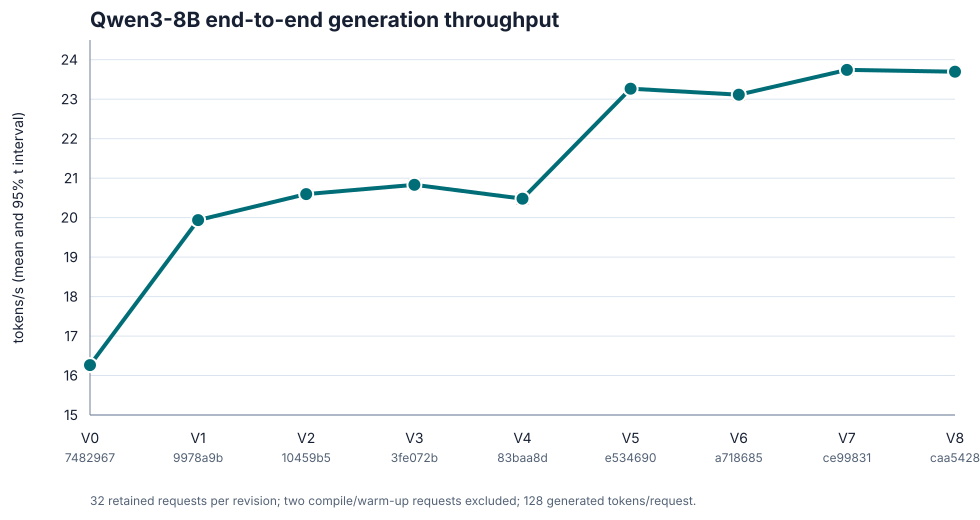
\includegraphics[width=1\textwidth,height=\textheight]{figures/throughput.svg}
\caption{Cumulative throughput across the measured
concepts.}\label{fig:throughput}
}
\end{figure}

\begin{figure}
\hypertarget{fig:incremental}{%
\centering
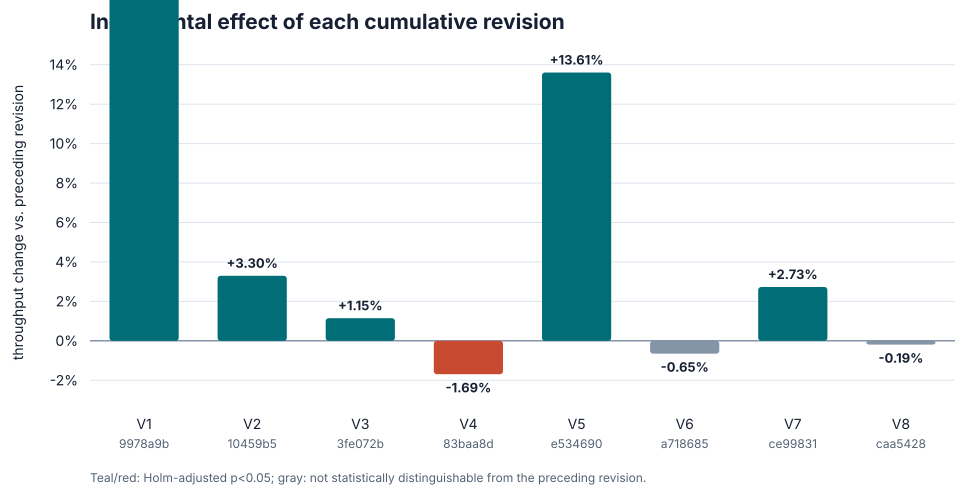
\includegraphics[width=1\textwidth,height=\textheight]{figures/incremental-speedup.svg}
\caption{Incremental effect of each concept in the established
sequence.}\label{fig:incremental}
}
\end{figure}

The negative and near-zero rows explain the final design: shared-LHS
fusion materializes too much data, consumer-side SiLU leaves the
producer boundary, and fallback removal changes coverage rather than the
kernel.

\hypertarget{current-kernel-ab-experiments}{%
\section{Current kernel A/B
experiments}\label{current-kernel-ab-experiments}}

\begin{longtable}[]{@{}lrcrr@{}}
\caption{Current-branch streaming results, 32 retained samples per
configuration. Width 4 is compared with width 2; the down projection is
compared with the same width-4 binary/configuration with the
specialization disabled.}\tabularnewline
\toprule
\begin{minipage}[b]{0.16\columnwidth}\raggedright
Configuration\strut
\end{minipage} & \begin{minipage}[b]{0.16\columnwidth}\raggedleft
Pure decode mean ± SD\strut
\end{minipage} & \begin{minipage}[b]{0.21\columnwidth}\centering
95\% CI\strut
\end{minipage} & \begin{minipage}[b]{0.16\columnwidth}\raggedleft
Streaming E2E mean ± SD\strut
\end{minipage} & \begin{minipage}[b]{0.16\columnwidth}\raggedleft
Change in decode\strut
\end{minipage}\tabularnewline
\midrule
\endfirsthead
\toprule
\begin{minipage}[b]{0.16\columnwidth}\raggedright
Configuration\strut
\end{minipage} & \begin{minipage}[b]{0.16\columnwidth}\raggedleft
Pure decode mean ± SD\strut
\end{minipage} & \begin{minipage}[b]{0.21\columnwidth}\centering
95\% CI\strut
\end{minipage} & \begin{minipage}[b]{0.16\columnwidth}\raggedleft
Streaming E2E mean ± SD\strut
\end{minipage} & \begin{minipage}[b]{0.16\columnwidth}\raggedleft
Change in decode\strut
\end{minipage}\tabularnewline
\midrule
\endhead
\begin{minipage}[t]{0.16\columnwidth}\raggedright
SwiGLU K block 2, generic down\strut
\end{minipage} & \begin{minipage}[t]{0.16\columnwidth}\raggedleft
26.122 ± 0.402\strut
\end{minipage} & \begin{minipage}[t]{0.21\columnwidth}\centering
{[}25.977, 26.267{]}\strut
\end{minipage} & \begin{minipage}[t]{0.16\columnwidth}\raggedleft
26.016 ± 0.396\strut
\end{minipage} & \begin{minipage}[t]{0.16\columnwidth}\raggedleft
---\strut
\end{minipage}\tabularnewline
\begin{minipage}[t]{0.16\columnwidth}\raggedright
SwiGLU K block 4, generic down\strut
\end{minipage} & \begin{minipage}[t]{0.16\columnwidth}\raggedleft
26.192 ± 0.338\strut
\end{minipage} & \begin{minipage}[t]{0.21\columnwidth}\centering
{[}26.071, 26.314{]}\strut
\end{minipage} & \begin{minipage}[t]{0.16\columnwidth}\raggedleft
26.085 ± 0.333\strut
\end{minipage} & \begin{minipage}[t]{0.16\columnwidth}\raggedleft
+0.27\%\strut
\end{minipage}\tabularnewline
\begin{minipage}[t]{0.16\columnwidth}\raggedright
K block 4, 110-core down\strut
\end{minipage} & \begin{minipage}[t]{0.16\columnwidth}\raggedleft
\textbf{27.753 ± 0.330}\strut
\end{minipage} & \begin{minipage}[t]{0.21\columnwidth}\centering
\textbf{{[}27.634, 27.872{]}}\strut
\end{minipage} & \begin{minipage}[t]{0.16\columnwidth}\raggedleft
\textbf{27.619 ± 0.322}\strut
\end{minipage} & \begin{minipage}[t]{0.16\columnwidth}\raggedleft
\textbf{+5.96\%}\strut
\end{minipage}\tabularnewline
\bottomrule
\end{longtable}

The down projection cuts mean decode time from 38.179 to 36.032
ms/token, a 2.147 ms/token saving. Streaming end-to-end throughput rises
by 5.88\%, from 26.085 to 27.619 tokens/s. TTFT remains about 58 ms.

\hypertarget{device-profile-of-the-down-projection}{%
\section{Device profile of the down
projection}\label{device-profile-of-the-down-projection}}

The direct TT-Metal profile identifies 36 occurrences per token,
matching the 36 Qwen3-8B decoder layers. Exactly those operation
positions change from 64 to 110 workers.

\begin{longtable}[]{@{}lrrr@{}}
\toprule
Metric & Generic program & 110-core specialization &
Change\tabularnewline
\midrule
\endhead
Workers & 64 & 110 & +71.9\%\tabularnewline
Mean kernel time/layer & 217.188 µs & 154.932 µs &
\textbf{-28.66\%}\tabularnewline
Effective BFP8 weight bandwidth & 246.2 GB/s & 345.2 GB/s &
\textbf{+40.18\%}\tabularnewline
Projected 36-layer saving & --- & 2.241 ms/token & ---\tabularnewline
\bottomrule
\end{longtable}

The projected kernel saving is close to the observed 2.147 ms/token. The
new program reaches about 92\% of the previously measured 375.1 GB/s
SwiGLU effective bandwidth. This agreement between operation profile and
end-to-end measurement supports the causal attribution.

\hypertarget{upstream-tt-inference-server-reference}{%
\section{Upstream tt-inference-server
reference}\label{upstream-tt-inference-server-reference}}

Tenstorrent's tt-inference-server is an OpenAI-compatible service built
around vLLM and TT-Transformers {[}25{]}. It enters the stack above TTNN
rather than through JAX, StableHLO, and TT-MLIR:

\begin{verbatim}
libtt:  SGLang-JAX → JAX/StableHLO → PJRT/TT-XLA/TT-MLIR → TTNN → TT-Metal
TTIS:   OpenAI API → vLLM → TT-Transformers                → TTNN → TT-Metal
\end{verbatim}

Both runs use the same P150, Qwen3-8B model, prompt, 128-token output,
serial request policy, disabled prefix cache, and persistent loopback
collector. Pure decode uses the 127 intervals from first to last token.
End-to-end throughput uses request send to last token. Each run has two
warm-ups and 32 retained requests.

\begin{longtable}[]{@{}lrrr@{}}
\toprule
\begin{minipage}[b]{0.22\columnwidth}\raggedright
Implementation\strut
\end{minipage} & \begin{minipage}[b]{0.22\columnwidth}\raggedleft
Pure decode mean ± SD {[}95\% CI{]} (tok/s)\strut
\end{minipage} & \begin{minipage}[b]{0.22\columnwidth}\raggedleft
Streaming E2E mean ± SD {[}95\% CI{]} (tok/s)\strut
\end{minipage} & \begin{minipage}[b]{0.22\columnwidth}\raggedleft
TTFT mean ± SD\strut
\end{minipage}\tabularnewline
\midrule
\endhead
\begin{minipage}[t]{0.22\columnwidth}\raggedright
libtt current (\texttt{37d5460})\strut
\end{minipage} & \begin{minipage}[t]{0.22\columnwidth}\raggedleft
\textbf{27.753 ± 0.330 {[}27.634, 27.872{]}}\strut
\end{minipage} & \begin{minipage}[t]{0.22\columnwidth}\raggedleft
\textbf{27.619 ± 0.322 {[}27.503, 27.735{]}}\strut
\end{minipage} & \begin{minipage}[t]{0.22\columnwidth}\raggedleft
\textbf{58.45 ± 1.50 ms}\strut
\end{minipage}\tabularnewline
\begin{minipage}[t]{0.22\columnwidth}\raggedright
TTIS v0.10.0\strut
\end{minipage} & \begin{minipage}[t]{0.22\columnwidth}\raggedleft
24.887 ± 0.532 {[}24.695, 25.079{]}\strut
\end{minipage} & \begin{minipage}[t]{0.22\columnwidth}\raggedleft
24.776 ± 0.524 {[}24.587, 24.964{]}\strut
\end{minipage} & \begin{minipage}[t]{0.22\columnwidth}\raggedleft
63.38 ± 2.10 ms\strut
\end{minipage}\tabularnewline
\bottomrule
\end{longtable}

\begin{figure}
\hypertarget{fig:upstream}{%
\centering
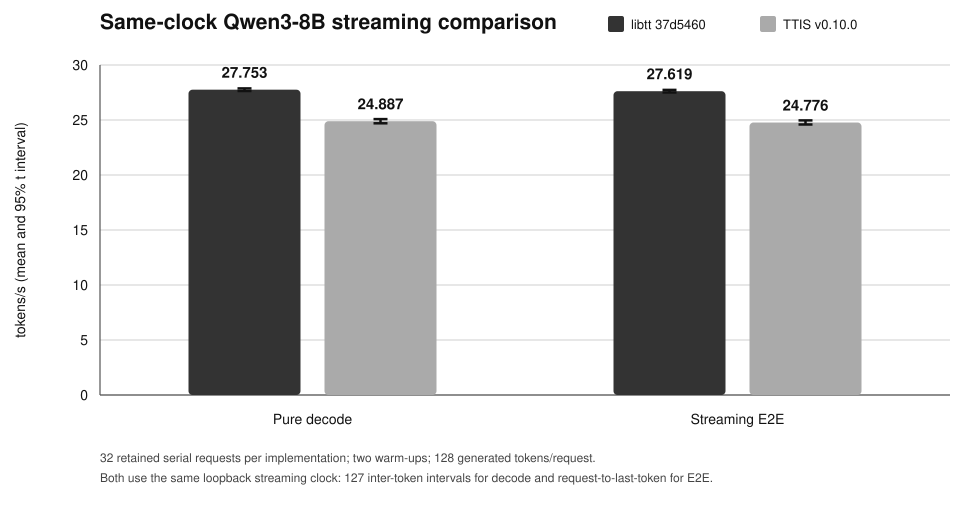
\includegraphics[width=1\textwidth,height=\textheight]{figures/upstream-comparison.svg}
\caption{External serving-stack reference on the same model
workload.}\label{fig:upstream}
}
\end{figure}

Current libtt is 11.51\% faster in pure decode and 11.48\% faster end to
end. Mean TTFT is 7.78\% lower, and mean request-to-last-token latency
falls from 5.169 to 4.635 seconds. This compares complete serving
stacks, not individual kernels; their model implementations, frontends,
and trace strategies differ. The tested TTIS artifact is the official
v0.10.0 runtime image.

\hypertarget{correctness-and-numeric-behavior}{%
\section{Correctness and numeric
behavior}\label{correctness-and-numeric-behavior}}

All 32 requests in each configuration are deterministic. Algebra and
reduction changes can alter the token hash. The current kernel hashes
are:

\begin{longtable}[]{@{}ll@{}}
\toprule
Configuration & SHA-256 prefix\tabularnewline
\midrule
\endhead
SwiGLU block 2, generic down & \texttt{5119e79e42b5}\tabularnewline
SwiGLU block 4, generic down & \texttt{c917933082e3}\tabularnewline
SwiGLU block 4, 110-core down & \texttt{c041ccb1901d}\tabularnewline
\bottomrule
\end{longtable}

Determinism and coherent text do not establish model quality. BF8
arithmetic, reassociation, and reduction order can change logits and
greedy choices. Perplexity and task-level evaluation are still required.

\hypertarget{engineering-rules}{%
\chapter{Engineering rules}\label{engineering-rules}}

\hypertarget{match-the-abstraction-to-the-information}{%
\section{Match the abstraction to the
information}\label{match-the-abstraction-to-the-information}}

Use each level for the information it retains:

\begin{itemize}
\tightlist
\item
  use \textbf{TTIR} when the problem is algebraic recognition or graph
  structure;
\item
  use \textbf{TTNN IR} when the compiler needs a named runtime
  operation, layout, or device dtype;
\item
  use the \textbf{TTNN runtime} when the choice depends on concrete
  tensor and device state;
\item
  use a \textbf{TT-Metal program factory} for core topology, circular
  buffers, multicast, and program selection; and
\item
  use \textbf{device kernels} for Dst lifetime, pack/unpack traffic,
  tile arithmetic, and synchronization.
\end{itemize}

Lower levels lose graph semantics; higher levels cannot control device
data movement.

\hypertarget{name-the-removed-boundary}{%
\section{Name the removed boundary}\label{name-the-removed-boundary}}

The MLP experiments remove different boundaries:

\begin{verbatim}
shared-LHS matmul:
  removes duplicate activation work, retains doubled output       → -1.69%

SiLU on BinaryNg input:
  removes one elementwise intermediate, retains matmul output     → -0.65%

matmul-SwiGLU epilogue:
  keeps gate/up in Dst and writes only the final half-width result → +2.73%
\end{verbatim}

Fusion should name the Dst, L1, DRAM, or launch boundary it removes.

\hypertarget{down-projection-geometry}{%
\section{Down-projection geometry}\label{down-projection-geometry}}

Profiling identified weight bandwidth as the down-projection limit.
Uneven N partitioning uses 110 workers without rereading weights or
reducing partials across cores. It reaches 345.2 GB/s with less
complexity than a 2D K/N split.

\hypertarget{keep-negative-results}{%
\section{Keep negative results}\label{keep-negative-results}}

Wider SwiGLU blocks reduce partial packs but add CB pressure or reduce
overlap. The four-tile result changes throughput by only +0.27\%, so two
remains the default and the larger values remain experimental.
Shared-LHS and consumer-side fusion are kept in the record for the same
reason: their measured costs explain the final producer-side design.

\hypertarget{limitations-and-follow-up-work}{%
\chapter{Limitations and follow-up
work}\label{limitations-and-follow-up-work}}

\begin{enumerate}
\def\labelenumi{\arabic{enumi}.}
\tightlist
\item
  \textbf{One model and decode regime.} Results apply to Qwen3-8B, a
  five-token prompt padded to one tile, serial 128-token generation, and
  a single P150. Other batches, contexts, and scheduling policies may
  have different limits.
\item
  \textbf{Cumulative attribution is ordered.} The established stages are
  real cumulative builds, not a factorial experiment. Patch effects can
  interact.
\item
  \textbf{The foundation group is not decomposed.} Its +22.58\% covers
  several compiler, dtype, validation, and layout changes.
\item
  \textbf{Two metric families.} The older cumulative sequence uses
  server-reported request latency. The current kernel and TTIS
  comparison uses the same streaming client clock. The two families are
  not directly interchangeable.
\item
  \textbf{Sequential sampling.} Configurations were not randomized or
  interleaved. Thermal and background drift can remain.
\item
  \textbf{Profile naming required positional alignment.} The final
  profiling CSV lacked operation names. Its 854 rows align with an
  earlier named trace, and the 36 changed positions match the down
  projections.
\item
  \textbf{Shape-specific kernels.} The 96-core epilogue and 110-core
  down projection target Blackhole and exact Qwen3-8B decode shapes.
\item
  \textbf{Quality is unmeasured.} Deterministic coherent completion is a
  smoke test, not evidence of equivalent perplexity or task accuracy.
\item
  \textbf{External reference scope.} The TTIS v0.10.0 image is official,
  but P150 model metadata was added locally because that release listed
  Qwen3-8B on P300. The runtime image was unchanged. Both rows use the
  same collector but different serving and model stacks.
\end{enumerate}

The next MLP experiment is to keep the SwiGLU output on chip for the
down projection. That requires a shared producer/consumer sharding
contract.

\hypertarget{reproduction-and-report-generation}{%
\chapter{Reproduction and report
generation}\label{reproduction-and-report-generation}}

The report directory contains:

\begin{itemize}
\tightlist
\item
  \texttt{report.md}: canonical source;
\item
  \texttt{data/samples.csv} and \texttt{data/summary.csv}: established
  32-sample sequence;
\item
  \texttt{data/current-kernel-samples.csv} and
  \texttt{data/current-kernel-summary.csv}: the blocking/down-projection
  A/B data;
\item
  \texttt{data/current-kernel-manifest.json}: exact current experiment
  provenance;
\item
  \texttt{data/down-projection-profile-summary.csv}: per-operation
  profile summary;
\item
  \texttt{data/latest-main-streaming-*}: direct prefill trace A/B data;
\item
  \texttt{data/upstream-tt-inference-*}: streaming TTIS observations,
  same-clock comparison statistics, and manifest;
\item
  \texttt{analyze.py}: statistics and SVG generation;
\item
  \texttt{benchmark\_upstream.py}: upstream reference collector;
\item
  \texttt{figures/*.svg}: vector figures; and
\item
  \texttt{Makefile} and \texttt{style.css}: HTML, LaTeX, and PDF
  generation.
\end{itemize}

To regenerate statistics when the raw \texttt{/tmp} benchmark
directories are available:

\begin{Shaded}
\begin{Highlighting}[]
\ExtensionTok{/home/pcmoritz/sglang{-}jax/.venv/bin/python} \KeywordTok{\textbackslash{}}
  \ExtensionTok{docs/libtt{-}optimization{-}report/analyze.py}
\end{Highlighting}
\end{Shaded}

To build a self-contained HTML report:

\begin{Shaded}
\begin{Highlighting}[]
\FunctionTok{make}\NormalTok{ {-}C docs/libtt{-}optimization{-}report html}
\end{Highlighting}
\end{Shaded}

To produce the typeset PDF with vector figures:

\begin{Shaded}
\begin{Highlighting}[]
\FunctionTok{make}\NormalTok{ {-}C docs/libtt{-}optimization{-}report pdf}
\end{Highlighting}
\end{Shaded}

The PDF build uses Pandoc, XeLaTeX, \texttt{booktabs},
\texttt{microtype}, and vector SVG conversion. Generated HTML, LaTeX,
and PDF files are versioned with the source.

\hypertarget{conclusion}{%
\chapter{Conclusion}\label{conclusion}}

\texttt{libtt.so} contains the PJRT backend, compiler, runtime, kernels,
and runtime assets. One Bazel graph pins and builds the stack, and its
patch surface reaches from TTIR graph rewrites to Tensix kernels.

The established changes improve Qwen3-8B end-to-end throughput by
60.61\%. The 110-core down projection adds 5.96\% pure decode
throughput, raises weight bandwidth by 40.2\%, and puts current libtt
11.51\% above the matched TTIS decode mean. These gains come from
changes at several levels: semantic recovery, layout policy, runtime
dispatch, core geometry, and device dataflow.

\hypertarget{bibliography}{%
\chapter*{Bibliography}\label{bibliography}}
\addcontentsline{toc}{chapter}{Bibliography}

\begin{enumerate}
\def\labelenumi{\arabic{enumi}.}
\tightlist
\item
  Tenstorrent, ``TT-XLA.'' \url{https://github.com/tenstorrent/tt-xla}
\item
  Tenstorrent, ``TT-MLIR.'' \url{https://github.com/tenstorrent/tt-mlir}
\item
  Tenstorrent, ``TT-NN Documentation.''
  \url{https://docs.tenstorrent.com/tt-metal/latest/ttnn/}
\item
  Tenstorrent, ``TT-Metalium Documentation.''
  \url{https://docs.tenstorrent.com/tt-metal/latest/tt-metalium/}
\item
  Tenstorrent, ``TT-UMD: User-Mode Driver for Tenstorrent Hardware.''
  \url{https://github.com/tenstorrent/tt-umd}
\item
  Tenstorrent, ``SFPI.'' \url{https://github.com/tenstorrent/sfpi}
\item
  Z. Tan, B. Kang, and A. Narasimham, ``A Developer's Guide to Debugging
  JAX on Cloud TPUs,'' Google Developers Blog, 2026. Describes
  \texttt{libtpu.so} as the shared library containing the XLA compiler,
  TPU driver, and hardware communication logic.
  \url{https://developers.googleblog.com/a-developers-guide-to-debugging-jax-on-cloud-tpus-essential-tools-and-techniques/}
\item
  Bazel Project, ``Hermeticity.''
  \url{https://bazel.build/concepts/hermeticity}
\item
  OpenXLA Project, ``PJRT---Uniform Device API.''
  \url{https://openxla.org/xla/pjrt}
\item
  OpenXLA Project, ``StableHLO Specification.''
  \url{https://openxla.org/stablehlo/spec}
\item
  C. Lattner et al., ``MLIR: Scaling Compiler Infrastructure for
  Domain-Specific Computation,'' \emph{2021 IEEE/ACM International
  Symposium on Code Generation and Optimization}, pp.~2--14, 2021.
  \url{https://doi.org/10.1109/CGO51591.2021.9370308}
\item
  Tenstorrent, ``TT-Forge: Open-Source AI Compiler Stack.''
  \url{https://github.com/tenstorrent/tt-forge}
\item
  Tenstorrent, ``TT-MLIR: Architecture and Dialect Overview.''
  \url{https://docs.tenstorrent.com/tt-mlir/overview.html}
\item
  Tenstorrent, ``TT-MLIR Tensor Layout.''
  \url{https://docs.tenstorrent.com/tt-mlir/specs/tensor-layout.html}
\item
  Tenstorrent, ``TT-Metalium Getting Started and Programming Model.''
  \url{https://docs.tenstorrent.com/tt-metal/latest/tt-metalium/get_started/get_started.html}
\item
  Tenstorrent, ``Compute Engines and Data Flow within Tensix.''
  \url{https://docs.tenstorrent.com/tt-metal/latest/tt-metalium/tt_metal/advanced_topics/compute_engines_and_dataflow_within_tensix.html}
\item
  Tenstorrent, ``Circular Buffer APIs.''
  \url{https://docs.tenstorrent.com/tt-metal/latest/tt-metalium/tt_metal/apis/kernel_apis/circular_buffers/circular_buffers.html}
\item
  Tenstorrent, ``Tiles.''
  \url{https://docs.tenstorrent.com/tt-metal/latest/tt-metalium/tt_metal/advanced_topics/tiles.html}
\item
  Tenstorrent, ``TTNN Tensor: Layout, Sharding, and BFLOAT8\_B.''
  \url{https://docs.tenstorrent.com/tt-metal/latest/ttnn/ttnn/tensor.html}
\item
  Tenstorrent, ``Blackhole PCIe Card Documentation'' and firmware
  release notes.
  \url{https://docs.tenstorrent.com/tt-system-firmware/boards/tenstorrent/tt_blackhole/doc/index.html}
\item
  SGLang Project, ``SGLang-JAX.''
  \url{https://github.com/sgl-project/sglang-jax}
\item
  A. Yang et al., ``Qwen3 Technical Report,'' arXiv:2505.09388, 2025.
  \url{https://arxiv.org/abs/2505.09388}
\item
  B. Zhang and R. Sennrich, ``Root Mean Square Layer Normalization,''
  \emph{Advances in Neural Information Processing Systems 32}, 2019.
  \url{https://proceedings.neurips.cc/paper/2019/hash/1e8a19426224ca89e83cef47f1e7f53b-Abstract.html}
\item
  N. Shazeer, ``GLU Variants Improve Transformer,'' arXiv:2002.05202,
  2020. \url{https://arxiv.org/abs/2002.05202}
\item
  Tenstorrent, ``tt-inference-server v0.10.0.''
  \url{https://github.com/tenstorrent/tt-inference-server/releases/tag/v0.10.0}
\end{enumerate}

\end{document}
